% !TEX program = pdflatex
% ------------------------------------------------------------
% ITKA2004 Databases & Data Management
% Lecture 1 (90 min): Course Introduction + Database Fundamentals
% Theme: metropolis
% ------------------------------------------------------------
\documentclass[10pt,aspectratio=169]{beamer}

\usetheme[
  progressbar=frametitle,
  numbering=fraction
]{metropolis}

% --- Packages
\usepackage[utf8]{inputenc}
\usepackage{booktabs}
\usepackage{amsmath}
\usepackage{tikz}
\usetikzlibrary{positioning,arrows.meta,shapes.geometric}

% ------------------------------------------------------------
% Make ALL included images automatically scale down to fit
% ------------------------------------------------------------
\usepackage{graphicx}
\setkeys{Gin}{width=\linewidth,height=0.70\textheight,keepaspectratio}

% ------------------------------------------------------------
% Footer (Metropolis)
% ------------------------------------------------------------
\setbeamertemplate{frame footer}{%
  \tiny Michael Emmerich (Professor, PS Fellow)\hfill Databases Spring 2026\hfill Faculty of Information Technology, University of Jyväskylä%
}

% --- Metadata
\title{Databases and Data Management}
\subtitle{Databases Spring 2026}
\author{Michael Emmerich (Professor, PS Fellow)}
\institute{Faculty of Information Technology\\University of Jyväskylä}
\date{Spring 2026}

% --- Title graphic
\titlegraphic{%
  \begin{tikzpicture}[remember picture,overlay]
    \node[anchor=south east,opacity=0.10] at ([xshift=-2mm,yshift=2mm]current page.south east) {%
      \begin{tikzpicture}[scale=0.75]
        \draw[rounded corners=6pt,line width=2pt] (0,0) rectangle (5,3);
        \draw[line width=2pt] (0.6,2.4) -- (4.4,2.4);
        \node at (2.5,1.6) {\Large DB};
      \end{tikzpicture}
    };
  \end{tikzpicture}%
}

\begin{document}

\maketitle

% ------------------------------------------------------------
\begin{frame}{Today (90 minutes)}
\begin{itemize}
  \item Course requirements (how to pass) + course structure
  \item What is a \textbf{database}? What is a \textbf{DBMS}?
  \item \textbf{Data models}: conceptual vs logical vs physical
  \item Data management: why it matters
  \item Mini activities + Q\&A
\end{itemize}
\end{frame}

% ------------------------------------------------------------
\section{Welcome \& why this course matters}

\begin{frame}{Welcome!}
\begin{itemize}
  \item Almost every application stores and uses data.
  \item Usually: application data lives in a \textbf{database}.
  \item Good data management improves:
    \begin{itemize}
      \item \textbf{security} (access control, backups, integrity),
      \item \textbf{performance} (fast queries, indexing),
      \item \textbf{reliability} (correctness under concurrent use).
    \end{itemize}
\end{itemize}
\end{frame}

\begin{frame}{Two systems, very different requirements}
\begin{columns}[T,onlytextwidth]
\column{0.48\textwidth}
\textbf{Simple note app}
\begin{itemize}
  \item Save, view, edit notes
  \item Small data volume
  \item Few users / low concurrency
\end{itemize}

\column{0.48\textwidth}
\textbf{Banking system}
\begin{itemize}
  \item Sensitive personal + financial data
  \item Backups, auditing, strict access control
  \item Thousands of transfers: balances must stay correct
  \item Strong consistency and transaction guarantees
\end{itemize}
\end{columns}
\end{frame}

\begin{frame}{Quick activity (2 minutes)}
\textbf{Think--pair--share:}
\begin{itemize}
  \item Name one app you used today that relies on a database.
  \item What is the \textbf{most important requirement} for its data?
\end{itemize}
\end{frame}

% ------------------------------------------------------------
\section{Course structure \& completion}

\begin{frame}{What you learn in this course}
You will learn:
\begin{itemize}
  \item key concepts: \textbf{database, CRUD, ACID, CAP}
  \item relational database skills: \textbf{ER diagrams, relations, SQL}
  \item data management topics: \textbf{data warehousing, distribution}
\end{itemize}
\end{frame}

\begin{frame}{Course structure (TIM sections)}
The course is divided into \textbf{five content areas} in TIM:
\begin{itemize}
  \item text material, examples, and exercises
  \item each section ends with a \textbf{mini-exam}
\end{itemize}

\vspace{0.5em}
Project work and the final exam instructions are in \textbf{Section 7}.
\end{frame}

\begin{frame}{How to pass (requirements)}
To pass the course, you must:
\begin{itemize}
  \item complete \textbf{every lecture revision test} (completion required; \textbf{score not graded})
  \item pass \textbf{every section mini-exam}
  \item submit \textbf{project work} by \textbf{15.3.2026}
  \item participate in the \textbf{course exam}
\end{itemize}

\vspace{0.35em}
\tiny Anonymized aggregates from revision tests may be used to estimate the class’ current level of understanding.
\end{frame}

\begin{frame}{Grading (1--5)}
Course grade is based on:
\begin{itemize}
  \item section mini-exams: \textbf{20\%}
  \item project work: \textbf{30\%}
  \item course exam: \textbf{50\%}
\end{itemize}

\vspace{0.5em}
Detailed schedules and criteria: \textbf{Section 1}.
\end{frame}

\begin{frame}{Lectures and recordings (Spring 2026)}
\begin{itemize}
  \item 9 lectures (English): \textbf{13.1.2026 -- 10.3.2026}, Tue \textbf{12:15--14:00}
  \item On-site: Agora \textbf{Ag B103 Auditorium 3} (capacity \(\approx\) 195)
  \item Attendence not mandatory. See it as a service if you prefer onsite lecture/interaction. Bring your laptop for participating in zoom polls.
  \item Remote: Zoom webinar (course link in TIM)
  \item Recordings available only to students registered via \textbf{Sisu}
\end{itemize}
\end{frame}

\begin{frame}{Support channels}
Official support:
\begin{itemize}
  \item Teachers' email list: \texttt{itka2004-teachers@jyu.onmicrosoft.com}
  \item Course Teams channel: Q\&A, announcements, guidance schedule
\end{itemize}

\vspace{0.5em}
Guidance:
\begin{itemize}
  \item Weekly lectures (9 lectures covering sections 1-6), you can ask questions to course instructor Prof. Emmerich in breaks or after lecture; hybrid format; attendance voluntarily.
  \item Course teacher email: michael.t.m.emmerich AT jyu.fi (please use [DB2026] in subject line.
\end{itemize}
\end{frame}

\begin{frame}{Workload (5 ECTS)}
\begin{itemize}
  \item 5 ECTS \(\approx\) \textbf{133 hours} total work
\end{itemize}

\begin{center}
\begin{tabular}{lr}
\toprule
\textbf{Activity} & \textbf{Hours} \\
\midrule
Lectures (9 x 1.5h) & 13.5 \\
Independent study (texts, examples) & \(\approx 51\) \\
Exercises & 35 \\
Project work & 13.5 \\
Weekly guidance (2h/week) & 20 \\
\midrule
\textbf{Total} & \textbf{133} \\
\bottomrule
\end{tabular}
\end{center}
\end{frame}

\begin{frame}{How to study efficiently}
\begin{enumerate}
  \item Skim the section
  \item Check the exercises and mini-exam scope
  \item Study examples with tasks in mind
  \item Do exercises; use model solutions to learn
  \item Ask in Teams / guidance sessions
\end{enumerate}
\end{frame}

% ------------------------------------------------------------
\section{Fundamentals: concepts and definitions}

\begin{frame}{Before databases: a very short history of information management}
\begin{itemize}
  \item \textbf{Ancient world:} clay tablets in Babylon/Mesopotamia, scribes, ledgers for trade, taxes, inventory
  \item \textbf{Libraries and archives:} cataloging, indexing, controlled vocabularies, hierarchical classification
  \item \textbf{Printing (Gutenberg, 15th century):} mass replication of records and standardized documents
  \item \textbf{20th century:} filing cabinets, punch cards, microfilm/microfiche, central registries
  \item \textbf{Early computer era:} file-based systems + early database models
    \begin{itemize}
      \item \textbf{hierarchical} (tree-structured records),
      \item \textbf{network} (graph-like links between records).
    \end{itemize}
\end{itemize}
\vspace{0.3em}
\small Key theme: the same needs keep returning --- \textbf{store, find, update, and trust} information at scale.
\end{frame}

\begin{frame}{Relational model: why it became dominant (and what came after)}
\begin{itemize}
  \item \textbf{Relational model (E. F. Codd, IBM, 1970):}
    \begin{itemize}
      \item data as \textbf{relations} (tables), with a precise mathematical foundation
      \item enables \textbf{declarative querying} and systematic optimization
    \end{itemize}
  \item \textbf{Conceptual modeling:} \textbf{ER model} (Peter Chen, 1976) to design databases from a domain view
  \item \textbf{Systems and adoption:}
    \begin{itemize}
      \item research prototypes and successors (e.g., \textbf{Ingres})
      \item commercial products (e.g., \textbf{Oracle}; founded by \textbf{Larry Ellison} and co-founders)
    \end{itemize}
  \item The relational database model became \textbf{predominant} in industry and remains foundational.
  \item \textbf{Afterwards:} distributed databases, data warehousing, and later \textbf{NoSQL} and NewSQL approaches.
\end{itemize}

\vspace{0.3em}
\alert{In this course we focus primarily on the relational model and its core tools: ER modeling, schema design, SQL, and normalization.}
\end{frame}

\begin{frame}{Key vocabulary for this course}
\begin{itemize}
  \item \textbf{Database}, \textbf{DBMS}, \textbf{database system}
  \item \textbf{Data model} (conceptual / logical / physical)
  \item \textbf{Schema} vs \textbf{instance}
  \item \textbf{Transaction}, \textbf{ACID}, \textbf{CAP}
  \item \textbf{CRUD} Create, Read, Update, Delete
\end{itemize}
\end{frame}

\begin{frame}{What is a database? (definition)}
A \textbf{database} is a collection of \textbf{related data}. Typically:
\begin{itemize}
  \item represents part of the \textbf{real world} (domain),
  \item is \textbf{logically coherent} (data has meaning through relationships),
  \item is \textbf{designed for a purpose} with intended users/applications.
\end{itemize}
\end{frame}

\begin{frame}{Database vs random data}
\textbf{Not a database:}
\begin{itemize}
  \item a folder of unrelated files,
  \item random numbers with no context.
\end{itemize}

\vspace{0.5em}
\textbf{Is a database:}
\begin{itemize}
  \item structured, coherent data with meaning and relationships,
  \item maintained as the domain changes.
\end{itemize}
\end{frame}

\begin{frame}{What is a DBMS?}
A \textbf{Database Management System (DBMS)} provides:
\begin{itemize}
  \item schema definition,
  \item search/insert/delete/update,
  \item security and maintenance,
  \item shared access for apps and users.
\end{itemize}
\end{frame}

\begin{frame}{Database system: the bigger picture}
\begin{columns}[T,onlytextwidth]
  \column{0.52\textwidth}
  A \textbf{database system} typically includes:
  \begin{itemize}
    \item the \textbf{database} (data + schema),
    \item the \textbf{DBMS},
    \item one or more \textbf{applications} (logic + UI).
  \end{itemize}

  \column{0.48\textwidth}
  \centering
  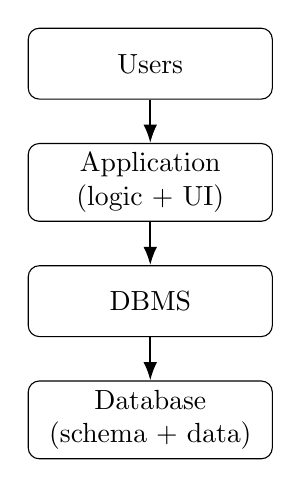
\begin{tikzpicture}[
    box/.style={draw,rounded corners,minimum width=3.1cm,minimum height=0.9cm,align=center},
    arr/.style={-Latex,thick}
  ]
    \node[box] (users) {Users};
    \node[box,below=0.55cm of users] (app) {Application\\(logic + UI)};
    \node[box,below=0.55cm of app] (dbms) {DBMS};
    \node[box,below=0.55cm of dbms] (db) {Database\\(schema + data)};

    \draw[arr] (users) -- (app);
    \draw[arr] (app) -- (dbms);
    \draw[arr] (dbms) -- (db);
  \end{tikzpicture}
\end{columns}
\end{frame}

\begin{frame}{Why SQLite in this course?}
\textbf{SQLite} is:
\begin{itemize}
  \item open-source and easy to start with,
  \item a \textbf{single-file} relational DBMS,
  \item widely used (browsers, mobile apps, IoT devices).
\end{itemize}
\end{frame}

% ------------------------------------------------------------
\section{Data models: how we think about data}

\begin{frame}{What is a data model?}
A \textbf{data model} defines:
\begin{itemize}
  \item data structures (e.g., relations/tables),
  \item operations (e.g., join),
  \item key concepts and constraints.
\end{itemize}
\end{frame}

\begin{frame}{Three levels: conceptual, logical, physical}
\begin{itemize}
  \item \textbf{Conceptual}: what information is needed? (e.g., ER)
  \item \textbf{Logical}: how is it organized for a DBMS paradigm? (e.g., relational)
  \item \textbf{Physical}: how is it stored? (indexes, storage layout)
\end{itemize}
\end{frame}

\begin{frame}{From domain to database: the modeling pipeline}
\begin{center}
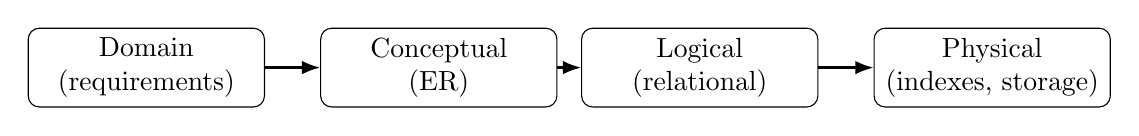
\begin{tikzpicture}[
  box/.style={draw,rounded corners,minimum width=3.0cm,minimum height=1.0cm,align=center},
  arr/.style={-Latex,thick}
]
\node[box] (domain) {Domain\\(requirements)};
\node[box,right=0.7cm of domain] (concept) {Conceptual\\(ER)};
\node[box,right=0.3cm of concept] (logical) {Logical\\(relational)};
\node[box,right=0.7cm of logical] (physical) {Physical\\(indexes, storage)};
\draw[arr] (domain) -- (concept);
\draw[arr] (concept) -- (logical);
\draw[arr] (logical) -- (physical);
\end{tikzpicture}
\end{center}
\end{frame}

\begin{frame}{Quick activity (3 minutes): pick the level}
Classify each statement:
\begin{enumerate}
  \item ``A customer can place many orders.''
  \item ``Table \texttt{Orders(order\_id, customer\_id, date)} with link to \texttt{Customers}.''
  \item ``Create an index on \texttt{Orders(customer\_id)}.''
\end{enumerate}
\end{frame}

% ------------------------------------------------------------
\section{Records, data, and data management}

\begin{frame}{What is a record?}
In databases, a \textbf{record} can refer to structured units such as:
\begin{itemize}
  \item a row (tuple, typically this is meant), column (related to field or attribute), table (relation), or even a whole database.
\end{itemize}
\end{frame}

\begin{frame}{Data vs information vs knowledge}
\begin{itemize}
  \item \textbf{Data}: raw values without context
  \item \textbf{Information}: data + context (meaning)
  \item \textbf{Knowledge}: information + perspective (significance)
\end{itemize}

\vspace{0.5em}
Example: ``1'' \(\rightarrow\) ``May 1'' \(\rightarrow\) ``May 1 is Vappu''.
\end{frame}

\begin{frame}{What is data management?}
Data management includes development, use, and governance to:
\begin{itemize}
  \item control and protect data,
  \item share data responsibly,
  \item increase data's value.
\end{itemize}
\end{frame}

% ------------------------------------------------------------
\section{Wrap-up}

\begin{frame}{Recap}
\begin{itemize}
  \item Database: related, meaningful, designed data about a domain
  \item DBMS: software to define, query, update, secure, and maintain data
  \item Data models: conceptual \(\rightarrow\) logical \(\rightarrow\) physical
  \item Data management: control, protection, sharing, value
\end{itemize}
\end{frame}

\begin{frame}{What to do before next lecture}
\begin{itemize}
  \item Complete the \textbf{Lecture 1 revision test} in TIM
  \item Join Teams for announcements and guidance schedules
  \item Skim the next section (ER modeling) and look at the exercises
\end{itemize}
\end{frame}

\begin{frame}{Q\&A}
\end{frame}

\begin{frame}{References}
\small
\begin{itemize}
  \item R. Elmasri, S. Navathe: \emph{Fundamentals of Database Systems}
\end{itemize}
\end{frame}

\end{document}
